%!TEX encoding = UTF-8 Unicode
%!TEX program = xelatex

\documentclass[doctor]{hnuthesis}
\usepackage{subfigure}  %插入多图时用子图显示的宏包
\usepackage{amsmath} % 提供更好的数学排版
\usepackage{algorithmicx,algpseudocode}
\usepackage{float}
\usepackage{pifont}
\usepackage{booktabs} % 提供更好的表格线  
\usepackage{setspace} % 调整行间距 
\usepackage{geometry} % 调整页面布局  
\usepackage{setspace} % 调整文档的行间距
\usepackage{makecell} % 设置表格单元格占用多行
\usepackage{multirow}  
\usepackage{array} % 对于更复杂的表格布局可能需要
\usepackage{booktabs}
\usepackage[export]{adjustbox} 

% \usepackage[backend=biber,style=gb7714-2015,gbalign=center]{biblatex}

\DeclareCaptionFont{myheiti}{\heiti\fontsize{10.5}{12.6}\selectfont} % 假设10.5pt近似于5号字体  
% 使用\captionsetup设置标题的字体样式  
\captionsetup{font={myheiti}}  

% https://blog.csdn.net/weixin_45893881/article/details/135082097
% \usepackage{ctex}
% \usepackage[backend=biber,style=gb7714-2015,gbpub=false]{biblatex}
% \addbibresource[location=local]{bibfile.bib} %注意这里bibfile.bib要替换成你的bib文件名


% 学校代码
\hnucode{10532}
% 学校名称
\hnuname{湖南大学}
\enhnuname{Hunan University}
% 中图分类号
\clc{TP391}         
% 密级
\secrettext{不保密}           

% 标题
\title{基于COTS的星载计算机软件冗余容错技术研究}
\entitle{Research on Software Redundancy and Fault Tolerance Technology of On-board Computer Based on COTS}
% 作者
\author{万孝国}
\enauthor{WAN Xiaoguo}
% \author{}
% \enauthor{}
% 学号
\authorid{S2110W0846}
% \authorid{}
% 学院
\college{信息科学与工程学院}
% 专业
\major{软件工程} 
\enmajor{Software Engineering}
%学士学位获得学校,年份
\enbachelor{B.E.~(Yanshan University)2021}
\endoctor{Master of engineering}
% 研究方向
\workon{冗余容错}
% 导师
\supervisor{张吉良教授、陈贤谋高级工程师}
\ensupervisor{Professor Zhang Jiliang}
\encosupervisor{Senior Engineer Chen Xianmou}
% \supervisor{}
% \ensupervisor{}
% \encosupervisor{}

% 论文提交、答辩日期
\submitdate{2024 年 05 月 3 日}
\defensedate{2024 年 05 月 21 日}
\defensedate{}
\endate{June, 2024}
% 答辩委员会主席
\chair{待定}


\begin{document}
% 封面、原创性声明
\maketitle

% 摘要
%中文摘要
\begin{abstract}
    摘要是论文内容的简要陈述,是一篇具有独立性和完整性的短文。摘要应包括本论文的创造性成果及其理论与实际意义。摘要中不宜使用公式、图表,不标注引用文献编号。避免将摘要写成目录式的内容介绍。
    注意不要头重脚轻
   
     关键词是供检索用的主题词条,应采用能覆盖论文主要内容的通用技术词条(参照相应的技术术语标准)。关键词一般列3~8个,按词条的外延层次排列(外延大的排在前面)。
       \keywords{关键词 1;关键词 2;关键词 3;关键词 4;关键词 5}
   \end{abstract}
   
   
   %英文摘要
   \begin{enabstract}
    Abstract is a brief statement of the content of the thesis, a short text with independence and completeness. The abstract should include the creative results of the thesis and its theoretical and practical significance. It is not appropriate to use formulas, graphs and charts in the abstract without citation numbers. Avoid writing the abstract as a table of contents presentation.
   
       \enkeywords{}
   \end{enabstract}
% 目录
\tableofcontents

% 插图附表索引
\begingroup
%latex在图表目录设置时自动识别章节并空出一定的间距
	\renewcommand*{\addvspace}[1]{}
	\newcommand{\loflabel}{图} 
	\renewcommand{\numberline}[1]{\loflabel~#1\hspace*{1em}}	
	\listoffigures
	\newcommand{\lotlabel}{表}
	\renewcommand{\numberline}[1]{\lotlabel~#1\hspace*{1em}}
	\listoftables
\endgroup


% 正文章节
\mainmatter

\chapter{绪论}
 引言(或绪论)一般作为第l章。引言(或绪论)应包括:本研究课题的学术背景及理论与实际意义;国内外文献综述;本研究课题的来源及主要研究内容。

\section{研究背景与意义}


\section{国内外研究现状分析}
\subsection{xxx}

最好,说明现有技术的问题,引出本文要采取什么样的技术路线。

\subsection{xxx}

\section{课题来源及主要研究内容}


\section{论文的组织结构}

%不需要本章小结
% \section{本章小结}

\chapter{相关理论基础}
[xxx]

\section{表格}

表应具有自明性。为使表格简洁易读,尽可能采用三线表,如表~\ref{tab:three-line}。

\begin{table}[H]
  \centering
  \caption{三线表示例}
  \begin{tabular}{ll}
    \toprule
    文件名          & 描述                         \\
    \midrule
    main.tex  & 入口文件 \\
    hnuthesis.cls   & 样式设置                     \\
    hnunumerical.bst & BibTeX 参考文献表样式文件    \\
    \bottomrule
  \end{tabular}
  \label{tab:three-line}
\end{table}

研究生要求使用英文小写字母 a、b、c……顺序编号。

\subsection{复杂一点}
latex 表格设置相对word 麻烦一些,比如表 ~\ref{table:test}。

\vspace{-10pt}
\begin{table}[H]  
\centering
\small
\caption{复杂一点点的表}
\label{table:test}  
\begin{tabular}{cccccccccc}  % 调整列数,以匹配内容  
\toprule  
\multicolumn{2}{c}{\multirow{3}{*}{\makecell[c]{目标}}} & \multicolumn{7}{c}{xxxx情况} & \multirow{3}{*}{$\beta$} \\  
\cline{3-9} % 在第3列到第6列之间划线  
 & & \makecell{项\\(1)} & \makecell{项\\(2)} & \makecell{项\\(3)} & \makecell{项\\(4)} & \makecell{项\\(5)} & \makecell{项\\(6)} & 项 & \\  
\midrule  
\multirow{3}{*}{\makecell[c]{任务1\\(xxx)}} & 子任务1 & 1 & 2 & 3 & 4 & 5 & 6 & 7 & 100\% \\  
 & 子任务2 & 1 & 2 & 3 & 4 & 5 & 6 & 7 & 100\% \\  
 & 子任务3 & 1 & 2 & 3 & 4 & 5 & 6 & 7 & 100\% \\  
 \multirow{3}{*}{\makecell[c]{任务1\\(xxx)}} & 子任务1 & 1 & 2 & 3 & 4 & 5 & 6 & 7 & 100\% \\  
 & 子任务2 & 1 & 2 & 3 & 4 & 5 & 6 & 7 & 100\% \\  
 & 子任务3 & 1 & 2 & 3 & 4 & 5 & 6 & 7 & 100\% \\  
\bottomrule  
\end{tabular}    
\end{table}  
\vspace{-10pt}

\section{图}

可以使用 pdf 格式的图,processon 能导出pdf,matplotlib 也能导出 pdf, 然后通过 pdfcandydt 进行裁剪。如图\ref{fig:img1}所示。

\vspace{-12pt}
\begin{figure}[H]
    \centering
    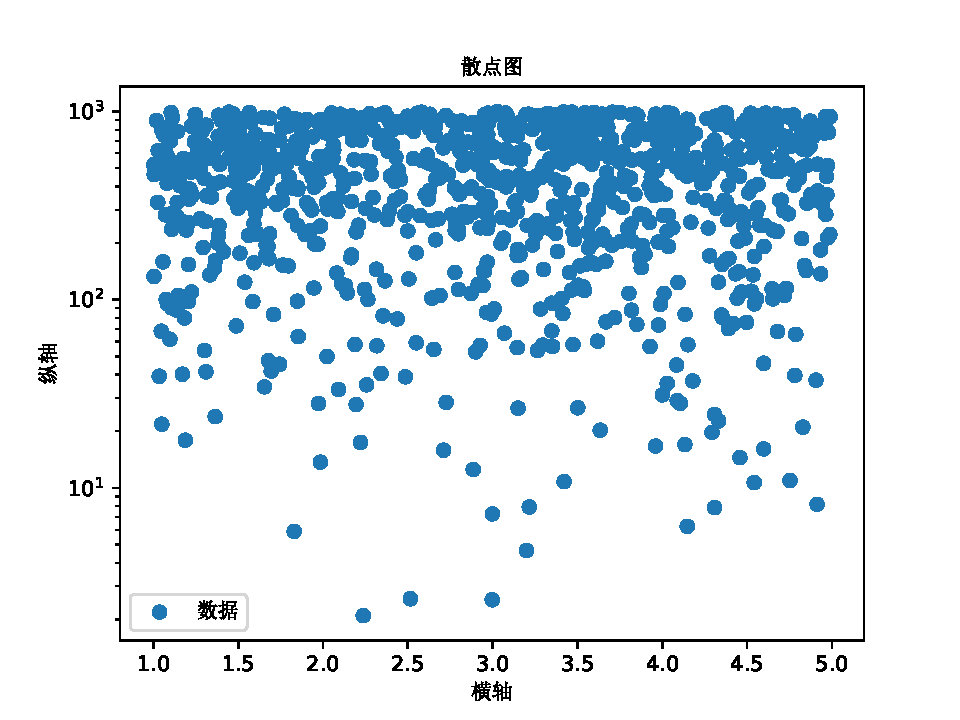
\includegraphics[width=0.6\linewidth]{figures/data/testA.pdf}
    \caption{图名}
    \label{fig:img1}
\end{figure}
\vspace{-18pt}

\subsection{子图}
如果一个图由两个或两个以上分图组成时,各分图分别以 (a)、(b)、(c)...... 作为图序,并须有分图题。
\begin{figure}[H] %这里使用的是强制位置,除非真的放不下,不然就是写在哪里图就放在哪里,不会乱动
	\centering  %图片全局居中
	\vspace{-0.35cm} %设置与上面正文的距离
	\subfigtopskip=2pt %设置子图与上面正文或别的内容的距离
	\subfigbottomskip=2pt %设置第二行子图与第一行子图的距离,即下面的头与上面的脚的距离
	\subfigcapskip=-5pt %设置子图与子标题之间的距离
	\subfigure[original]{
		\label{level.sub.1}
		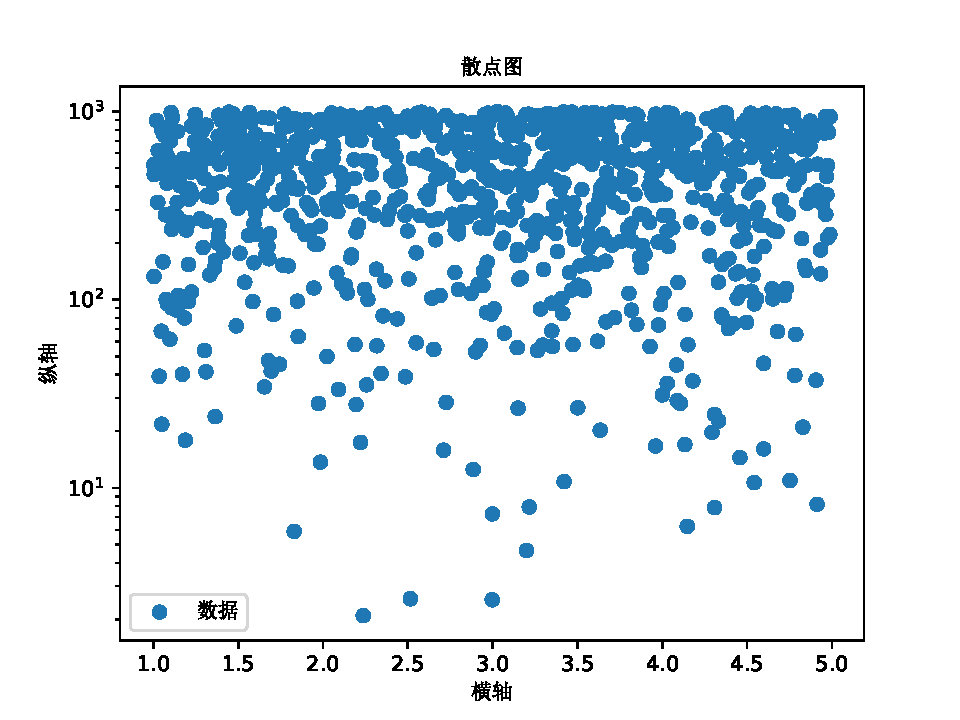
\includegraphics[width=0.45\linewidth]{figures/data/testA.pdf}}
	\quad %默认情况下两个子图之间空的较少,使用这个命令加大宽度
	\subfigure[level=9]{
		\label{level.sub.2}
		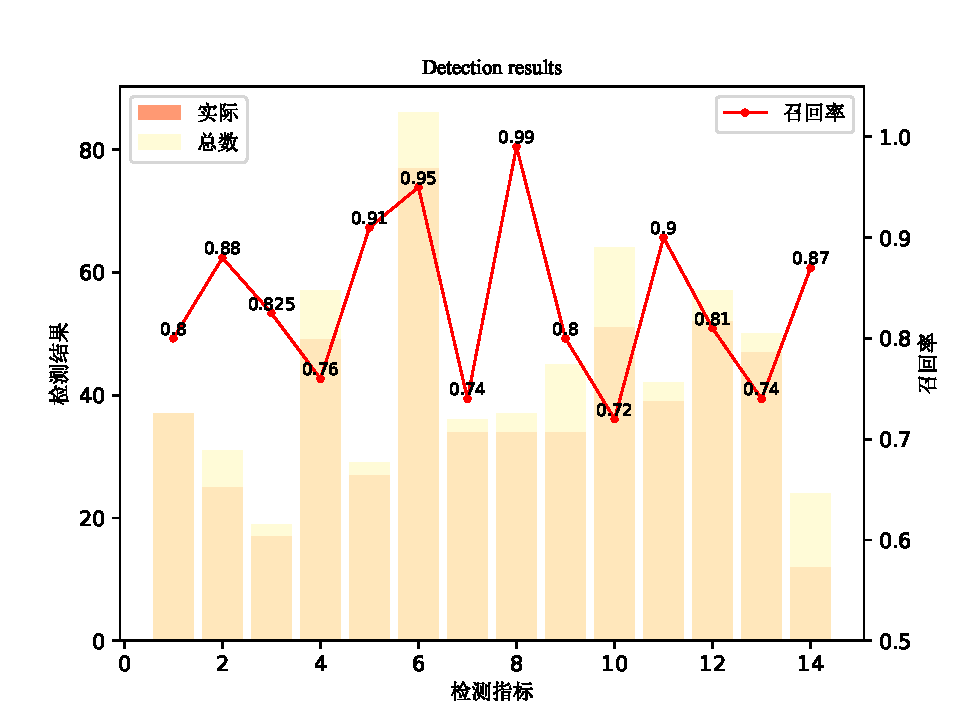
\includegraphics[width=0.45\linewidth]{figures/data/testB.pdf}}
	  %这里是空了一行,能够实现强制将四张图分成两行两列显示,而不是放不下图了再换行,使用\\也行。
	\caption{子图}
	\label{level}
\end{figure}

\section{公式}

行内公式,$p = q * \frac{q}{p}$,$\begin{bmatrix} a & b & c \end{bmatrix}$。

单行公式。

\begin{equation}
    e = \lim_{n\to \infty} \left(1 + \frac{1}{n}\right)^n
\end{equation}

多行公式~\ref{eq:foo}。

\begin{equation}
    \begin{aligned}
        1+ 1*2 - (2-1) & = 1+ 2 - 1 \\
                       & = 3-1      \\
                       & = 2
    \end{aligned}
    \label{eq:foo}
\end{equation}

多行公式,每行带序号
\begin{align}
  a & = b + c + d + e \\
    & = f + g
\end{align}


多行公式(无序号)。

\begin{equation*}
    \begin{aligned}
        1+ 1*2 - (2-1) & = 1+ 2 - 1 \\
                       & = 3-1      \\
                       & = 2
    \end{aligned}
\end{equation*}



\section{算法}

算法环境可以使用 \textbf{algorithms} 或者  \textbf{algorithm2e} 宏包。

\renewcommand{\algorithmicrequire}{\textbf{输入:}\unskip}
\renewcommand{\algorithmicensure}{\textbf{输出:}\unskip}



\section{本章小结}


\chapter{创新点1}
[xxx]

\section{第一节}

\subsection{第一小节}

\subsubsection{第一小小节}


% normalsize
{\large\ding{192}} 1

{\large\ding{193}} 2

{\large\ding{194}} 3


\section{本章小结}

\chapter{创新点2}
[xxx]

\section{xxx}



\section{本章小结}

% \input{chapters/ch5}
\begin{summary}
    学位论文的结论单独作为一章排写,但不加章号。
    
        结论是对整个论文主要成果的总结。在结论中应明确指出本研究内容的创造性成果或创新性理论(含新见解、新观点),对其应用前景和社会、经济价值等加以预测和评价,并指出今后进一步在本研究方向进行研究工作的展望与设想。结论内容一般在2000字左右(以汉字计)。
    
    \end{summary}
    
\bibliography{references}
% \printbibliography[heading=bibliography,title=参考文献]
% 附录
\appendix
\chapter{读学位期间所发表的成果}

\begin{enumerate}
	\renewcommand{\labelenumi}{[\theenumi]}
    \item 软件著作权一篇,导师第一,本人第二
    \item ITC-Asia2024 论文在投,本人第一
\end{enumerate}

\chapter{读学位期间所参加的科研项目}

\begin{enumerate}
	\renewcommand{\labelenumi}{[\theenumi]}
	\item 某某课题
\end{enumerate}


% 致谢
\backmatter
\begin{acknowledgements}
    对导师和给予指导或协助完成学位论文工作的组织和个人表示感谢。内容应简洁明了、实事求是。对课题给予资助者应予感谢。
 
 \end{acknowledgements}
 

\end{document}

